\documentclass[10pt]{beamer}
\usefonttheme{professionalfonts,serif}
\def\newblock{\hskip .11em plus .33em minus .07em}
\usepackage[numbers,sort]{natbib}
\renewcommand{\rmdefault}{psbx}
\usepackage[utf8]{inputenc}
\usepackage[T1]{fontenc}
\usepackage{textcomp}
\usepackage{eulervm}

\usetheme{default}           % tips from David Blei
\useinnertheme{circles}
\useoutertheme{infolines}
\setbeamertemplate{headline}{}
\setbeamertemplate{navigation symbols}{}
\setbeamerfont{itemize/enumerate subbody}{size=\normalsize}
\setbeamerfont{itemize/enumerate subsubbody}{size=\normalsize}
\usecolortheme{seahorse}
\setbeamersize{text margin left=2mm,text margin right=2mm}

\graphicspath{{../../figures/}}

\definecolor{mypine}{rgb}{0.05,0.45,0.05}
\definecolor{mycyan}{rgb}{0.0,0.9,0.9}
\newcommand{\Red}{\textcolor{red}}
\newcommand{\Blue}{\textcolor{blue}}
\newcommand{\Green}{\textcolor{mypine}}
\newcommand{\PineGreen}{\textcolor{mypine}}
\newcommand{\Magenta}{\textcolor{magenta}}
\newcommand{\Cyan}{\textcolor{mycyan}}

\newcommand{\N}{\mathcal{N}}
\newcommand{\R}{\mathbb{R}}
\newcommand{\T}{{\scriptsize^{\top}}}
\newcommand{\D}{\mathcal{D}}
\newcommand{\F}{\mathcal{F}}
\newcommand{\E}{\mathbb{E}}
\newcommand{\V}{\mathbb{V}}
\newcommand{\M}{\mathcal{M}}
\newcommand{\KL}{\mathcal{KL}}
\newcommand{\cut}[1]{}
\newcommand{\trace}{\operatorname{trace}}

\newcommand{\bmu}{{\boldsymbol{\mu}}}
\newcommand{\btheta}{\boldsymbol{\theta}}
\newcommand{\bepsilon}{\boldsymbol{\epsilon}}
\newcommand{\balpha}{\boldsymbol{\alpha}}
\newcommand{\bbeta}{\boldsymbol{\beta}}
\newcommand{\bphi}{\boldsymbol{\phi}}
\newcommand{\bPhi}{\boldsymbol{\Phi}}
\newcommand{\bSigma}{\boldsymbol{\Sigma}}
\newcommand{\bpi}{\boldsymbol{\pi}}
\newcommand{\blambda}{\boldsymbol{\lambda}}

\newcommand{\argmax}{\operatorname{argmax}}
\newcommand{\argmin}{\operatorname{argmin}}
\newcommand{\ci}{{\bot\negthickspace\negthickspace\bot}} % conditional indep.
\newcommand{\neigh}{\operatorname{ne}}
\newcommand{\vectr}[2]{  \left[ \!\!\begin{array}{c} #1 \\
      #2 \end{array} \!\!\right]}
\newcommand{\deff}{\stackrel{\mathrm{def}}{=}}
\newcommand{\deldel}[2]{\frac{\partial #1}{\partial #2}}

\newcommand{\maketilde}{\raisebox{0.4ex}{\tiny $\sim$}}
\newcommand{\bfa}{\mathbf a}
\newcommand{\bfb}{\mathbf b}
\newcommand{\bfe}{\mathbf e}
\newcommand{\bff}{\mathbf f}
\newcommand{\bfk}{\mathbf k}
\newcommand{\bfm}{\mathbf m}
\newcommand{\bfn}{\mathbf n}
\newcommand{\bfp}{\mathbf{p}}
\newcommand{\bfs}{\mathbf s}
\newcommand{\bfu}{\mathbf u}
\newcommand{\bfx}{\mathbf x}
\newcommand{\bfy}{\mathbf y}
\newcommand{\bft}{\mathbf t}
\newcommand{\bfv}{\mathbf v}
\newcommand{\bfw}{\mathbf w}
\newcommand{\bfA}{\mathbf A}
\newcommand{\bfI}{\mathbf I}
\newcommand{\bfK}{\mathbf K}


\title{Marginal Likelihood}
\author{Carl Edward Rasmussen}
\date{July 1st, 2016}

\begin{document}

\begin{frame}
\titlepage
\end{frame}

\begin{frame}
\frametitle{Key concepts}

\end{frame}


\begin{frame}
\frametitle{Marginal likelihood}
\[
\Green{p({\bf w}|{\bf x},{\bf y},\mathcal{M})}\;=\;\frac{\Blue{p({\bf w}|\mathcal{M})}
\Red{p({\bf y}|{\bf x},{\bf w},\mathcal{M})}}{\Cyan{p({\bf y}|{\bf x},\mathcal{M})}}
\]

{\bf Marginal likelihood:}
\[
\Cyan{p({\bf y}|{\bf x},\mathcal{M})}\;=\;
\int\Blue{p({\bf w}|\mathcal{M})}\Red{p({\bf y}|{\bf x},{\bf w},\mathcal{M}})d{\bf w}.
\]

Second level inference: model comparison and Bayes' rule again
\[
p(\mathcal{M}|{\bf y},{\bf x})\;=\;\frac{\Cyan{p({\bf y}|{\bf
      x},\mathcal{M})} p(\mathcal{M})}{p({\bf y}|{\bf x})}
\;\propto\;\Cyan{p({\bf y}|{\bf x},\mathcal{M})}p(\mathcal{M}).
\]
The \Cyan{\emph{marginal likelihood}} is used to select between models.

For linear in the parameter models with Gaussian priors and noise:
\[
\Cyan{p({\bf y}|{\bf x},\mathcal{M})} \;=\;
\int\Blue{p({\bf w}|\mathcal{M})}\Red{p({\bf y}|{\bf x},{\bf w},\mathcal{M}})d{\bf w}
\;=\; \N(\bfy;\;\mathbf{0},\sigma_\bfw^2\,\bPhi\,\bPhi^\top+\sigma_\mathrm{noise}^2\,\bfI)
\]

\end{frame}


\begin{frame}
\frametitle{Understanding the marginal likelihood (1). Models}

Consider 3 models $\mathcal{M}_1$,  $\mathcal{M}_2$ and  $\mathcal{M}_3$. Given our data:
\begin{itemize}
\item We want to compute the \Blue{\emph{marginal likelihood}} for each model.
\item We want to obtain the predictive distribution for each model.
\end{itemize}
\vspace{-0.5cm}
\parbox{\textwidth}{
\centerline{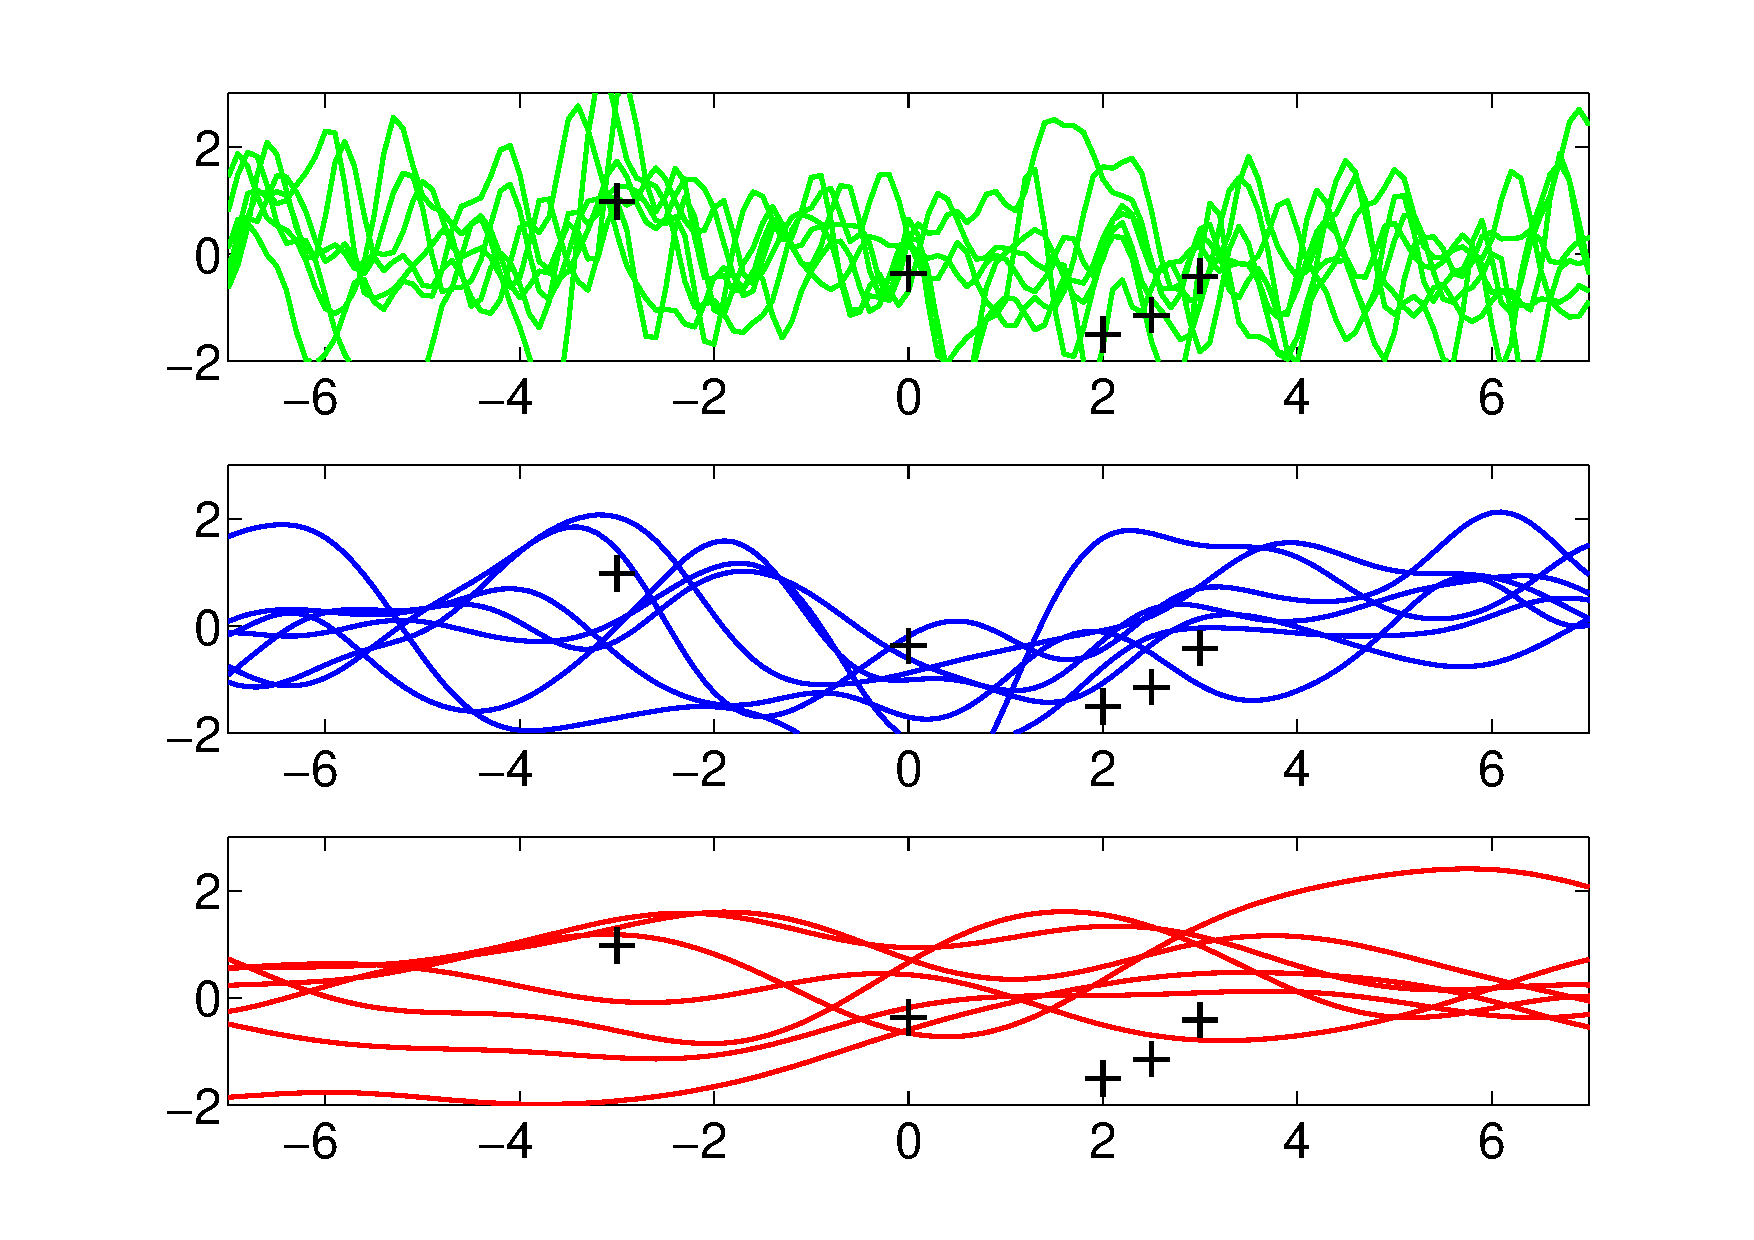
\includegraphics[width=0.8\textwidth]{rejection_sampling_data_priors.pdf}}
}

\end{frame}


\begin{frame}
\frametitle{Understanding the marginal likelihood (2). Noise}

Consider a very simple noise model for $y_n = f(x_n) + \epsilon_n$
\begin{itemize}
\item $\epsilon_n\sim\mathrm{Uniform}(-0.2, 0.2)$ and all noise terms are independent.
\[
p(y_n|f(x_n))= \left\{ 
\begin{array}{ll}  0 & \mathrm{if\; } |y_n-f(x_n)|>0.2\\
  1/0.4=2.5 &  \mathrm{otherwise}
\end{array}
 \right.
\]
\item The likelihood of a given function from the prior is 
%
\[
p(\bfy|\bff)=\prod_{n=1}^Np(y_n|f(x_n))=
\left\{
\begin{array}{ll}
0 &\mathrm{if\;for\;any\;}n, \; |y_n-f(x_n)|>0.2 \\
2.5^N &\mathrm{otherwise}
\end{array}
\right.
\]
%
\end{itemize}

We will approximate the marginal likelihood by \Blue{\emph{Monte
    Carlo}} sampling:
%
\[
p(\bfy|\mathcal{M}_i)=\int p(\bfy|\bff)\,p(\bff|\mathcal{M}_i)\,\mathbf{\mathrm{d}}\,\bff
\approx \frac{1}{S}\sum_{s=1}^{S} p(\bfy|\bff_s) = \frac{S_a}{S}\cdot2.5^N
\]
%
\vspace*{-2ex}
\begin{itemize}
\item A total of $S$ functions are sampled from the prior $p(\bff|\mathcal{M}_i)$. 
\item $\bff_s$ is the $s^\mathrm{th}$ function sampled from the prior.
\item $S_a$ is the number of samples with non-zero likelihood: these are accepted. The 
remaining $S-S_a$ samples are rejected.
\end{itemize}

\end{frame}



\begin{frame}
\frametitle{Simple Monte Carlo}

We can approximate integrals of the form
\[
z\;=\;\int f(x) p(x) dx,
\]
where $p(x)$ is a probability distribution, using a sum
\[
z\;\simeq\frac{1}{T}\sum_{t=1}^T f(x^{(t)}),\text{\ \ where\ \ }x^{(t)}\sim p(x).
\]
As $T\rightarrow \infty$ the approximation (under very mild conditions)
converges to $z$.

This algorithm is called \Blue{\emph{Simple Monte Carlo}}.
\end{frame}


\begin{frame}
\frametitle{Understanding the marginal likelihood (3). Posterior}

\Blue{\emph{Posterior samples}} for each of the models obtained by rejection sampling.
\begin{itemize}
\item For each model we draw 1 million samples from the prior.
\item We only keep the samples that have non-zero likelihood.
\end{itemize}
\vspace{-0.5cm}
\parbox{0.18\textwidth}
{
%
\vspace{-0.6cm}
\[
\begin{array}{r|l}
S_a & p(\bfy|\mathcal{M}_i)\\
\hline\\
8 & 8 \times 10^{-4}\\[1.65cm]
\mathbf{88} & \mathbf{9 \times 10^{-3}}\\[1.65cm]
17 & 2\times 10^{-3}
\end{array}
\]
%
}
\parbox{0.81\textwidth}
{
\centerline{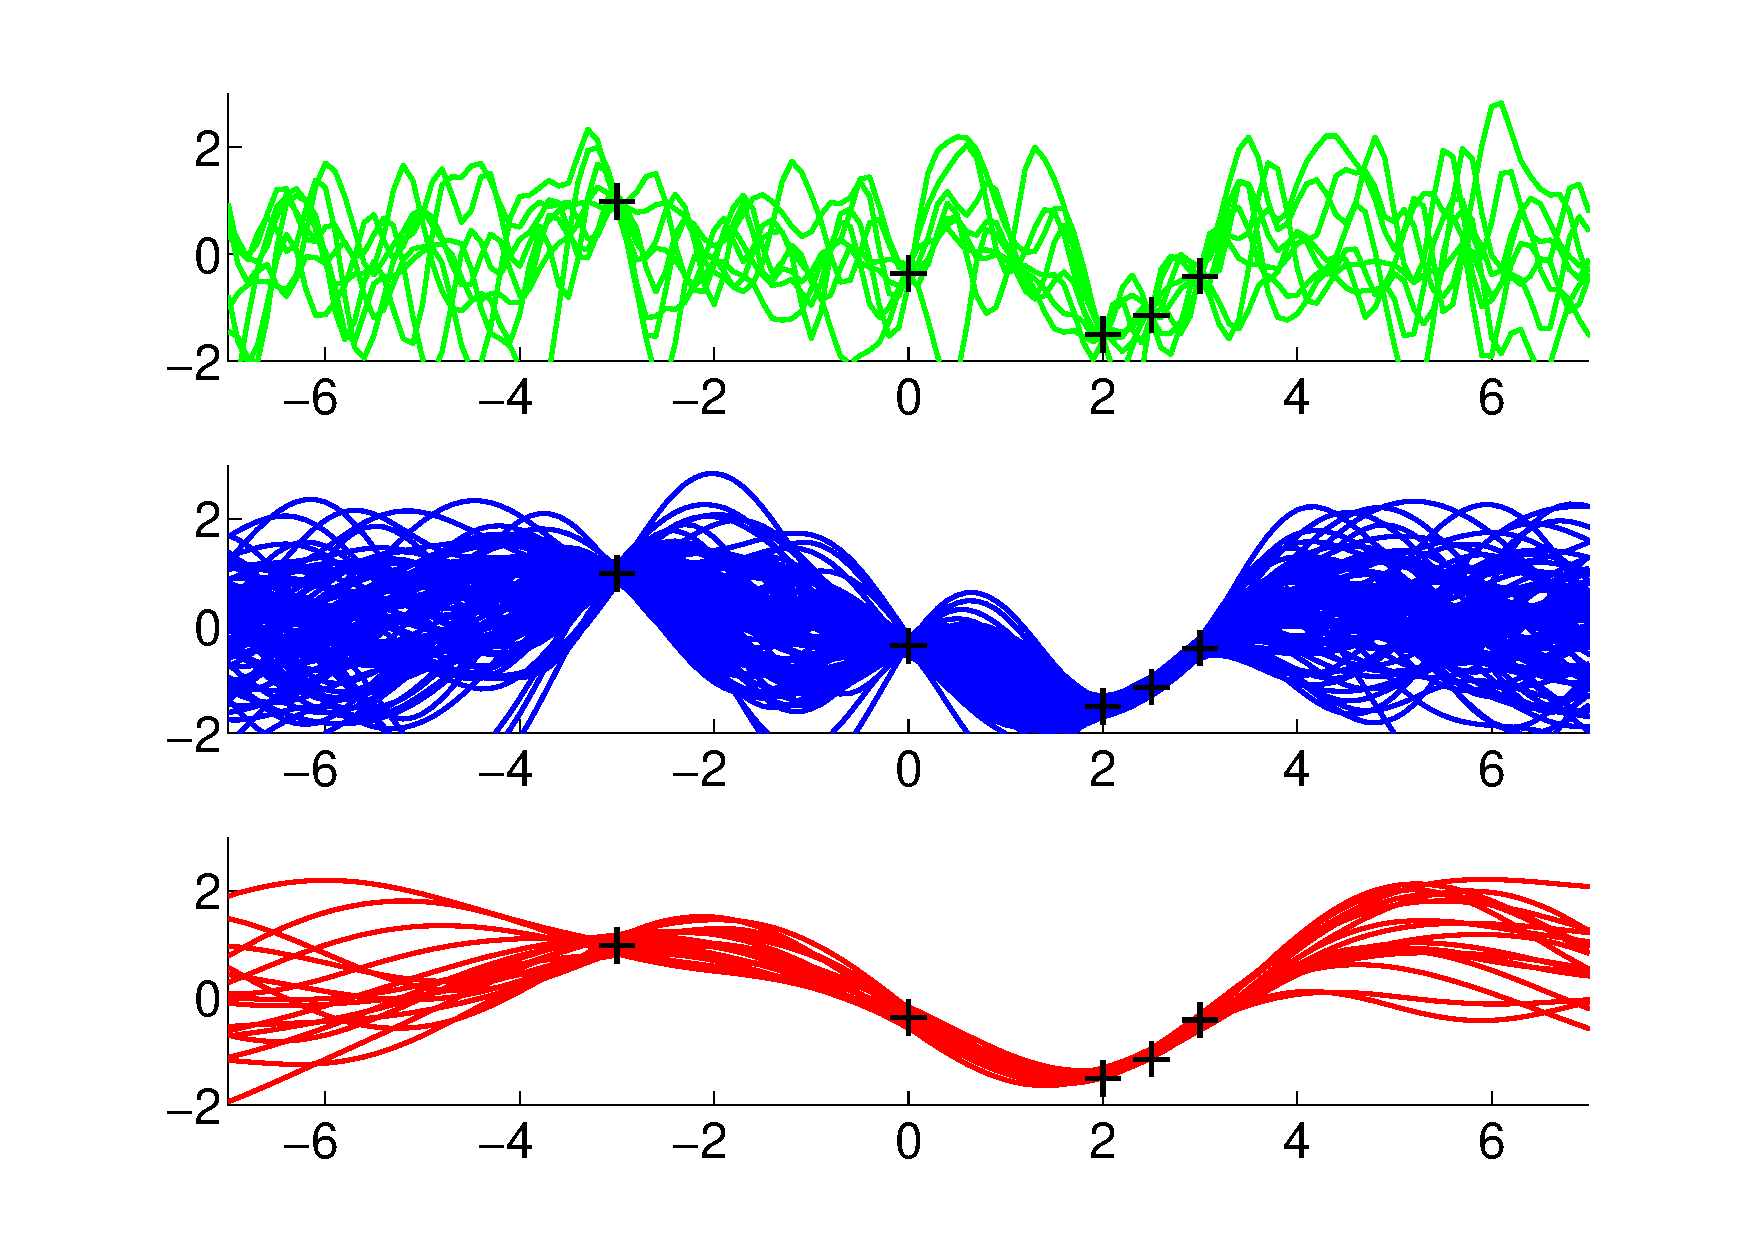
\includegraphics[width=0.8\textwidth]{rejection_sampling_data_posteriors.pdf}}
}


\end{frame}
\begin{frame}
\frametitle{Predictive distribution}

\Blue{\emph{Predictive distribution}} for each of the models obtained.
\begin{itemize}
\item For each model we take all the posterior functions from rejection sampling.
\item We compute the average and standard deviation of $f_s(x)$.
\end{itemize}
\vspace{-0.5cm}
\parbox{\textwidth}{
\centerline{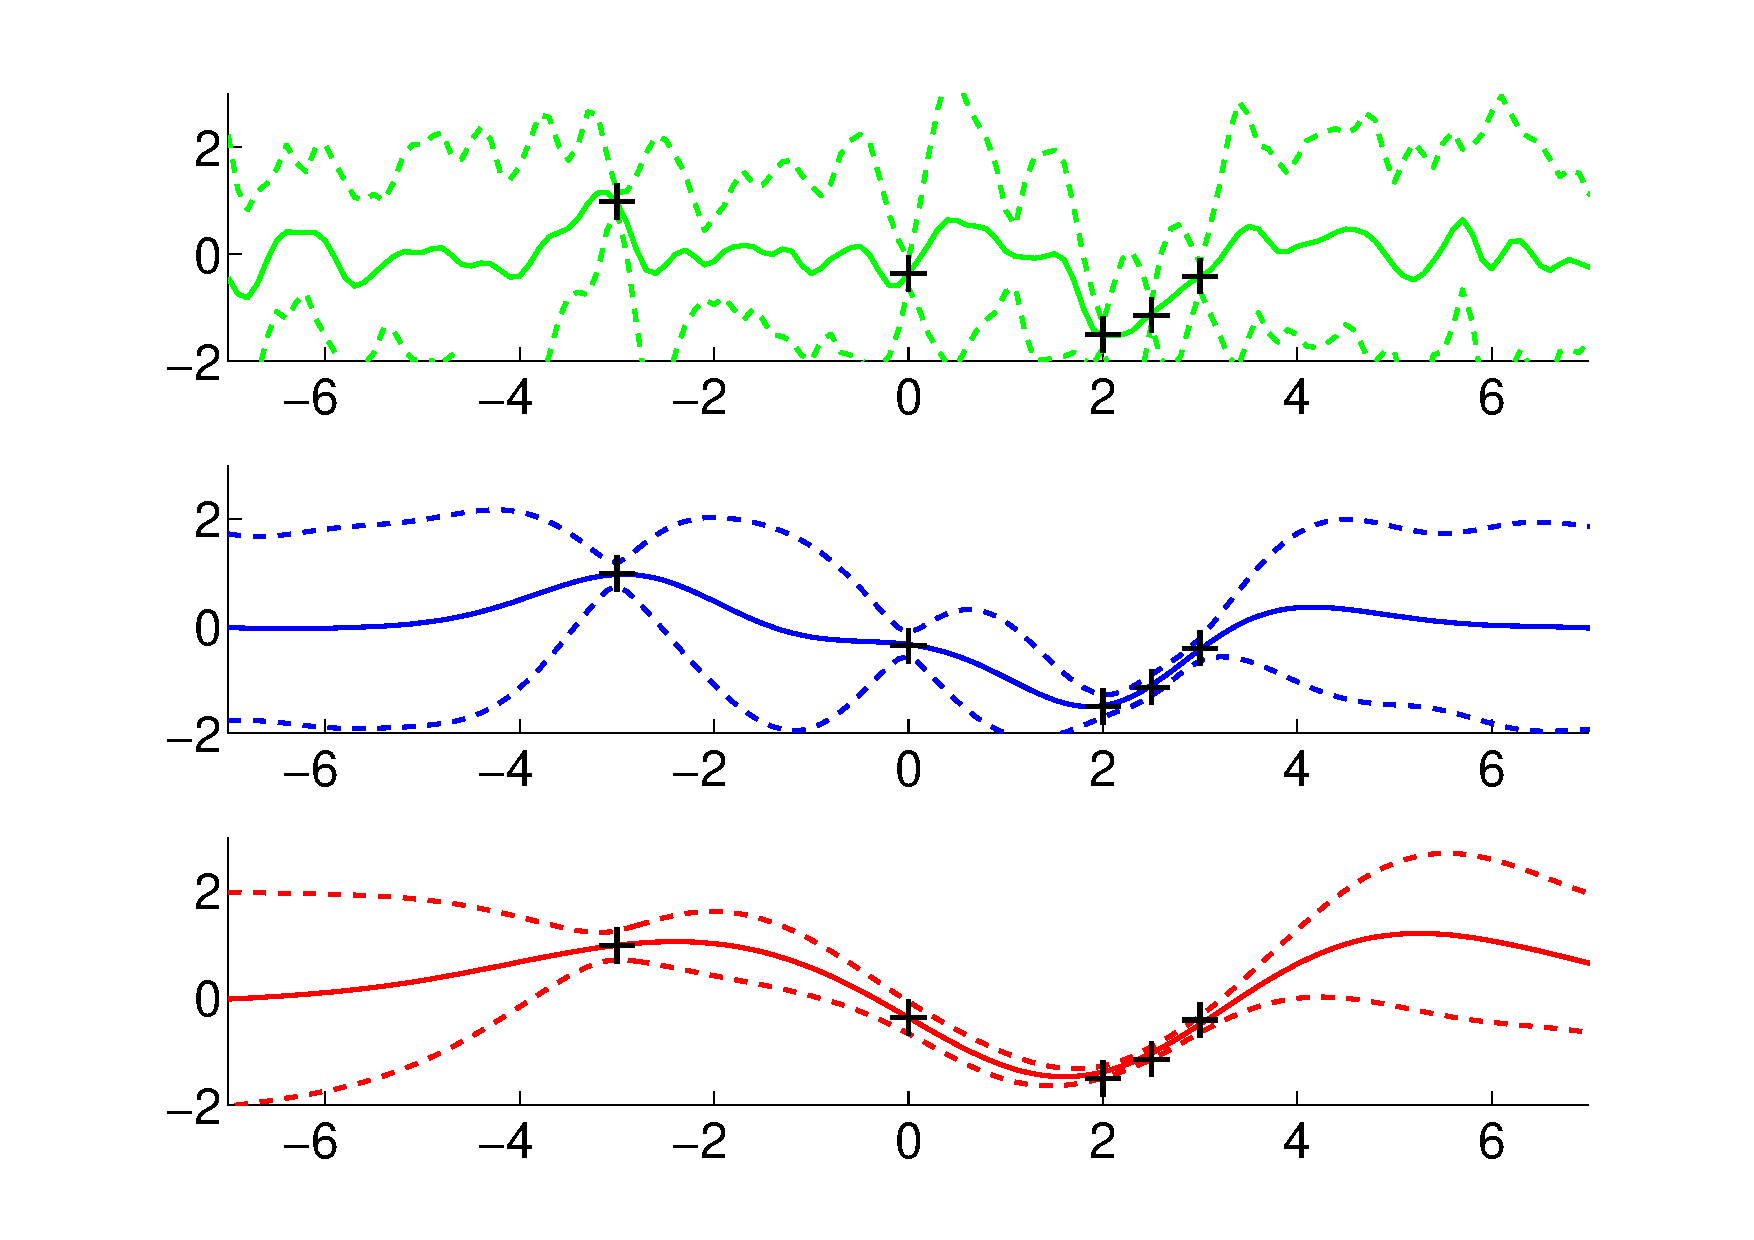
\includegraphics[width=0.8\textwidth]{rejection_sampling_predictive_distributions.pdf}}
}
\end{frame}


\begin{frame}
\frametitle{Conclusions}
Probability theory provides a framework for
\begin{itemize}
\item making inferences from data in a model
\item making probabilistic predictions
\end{itemize}

It also provides a \Blue{\emph{principled}} and \Blue{\emph{automatic}} way of doing
\begin{itemize}
\item model comparison
\end{itemize}

In the following lectures, we'll demonstrate how to use this framework
to solve challenging machine learning problems.
\end{frame}

\end{document}